\documentclass[12pt,letterpaper]{article}

\PassOptionsToPackage{hyphens}{url}
\usepackage[pdftex, bookmarksopen=true, bookmarksnumbered=true,
pdfstartview=FitH, breaklinks=true, urlbordercolor={0 1 0}, citebordercolor={0 0 1}]{hyperref}

% === MARGINS ===
\addtolength{\hoffset}{-0.75in} \addtolength{\voffset}{-1.25in}
\addtolength{\textwidth}{1.5in} \addtolength{\textheight}{2.25in}

% == ENVS ==
\newenvironment{tightcenter}{%
  \setlength\topsep{0pt}
  \setlength\parskip{0pt}
  \begin{center}
}{
  \end{center}
}

% == PACKS ==
\usepackage{color,soul}
\usepackage{graphicx}
\usepackage{calc} % To scale \pagewidth with \real{float}
\usepackage{pgfplots} % To draw histogram
\pgfplotsset{compat=1.17} % request specific version of pgfplots
\usepackage{calc} % to use \real for text -> numeric
\usepackage{pgf} % to store numeric variables
\usepackage{subcaption} % to place two figures horizontally
\usepackage{tikz}
\usetikzlibrary{automata,positioning}
\usetikzlibrary{arrows.meta, positioning, automata}
\tikzset{
  font={\fontsize{10pt}{0}\selectfont}}
\usepackage{forest}
\tikzset{
  Decision/.style = {%
    draw,
    line width=1.4pt
  },
  Lottery/.style = {%
    draw,
    line width=1.4pt
  },
  Outcome/.style = {%
    circle,
    minimum width=3pt,
    fill,
    inner sep=0pt
  }
}


  % == BIBS ==
\usepackage{natbib}
\bibliographystyle{apsr}

% == SPACES == 

% == CMMDS ==
\newcommand{\tit}{
\bf 
Mapping Regulatory Network of WTO Dispute Settlement Body Using Deep Learning
}
\newcommand\spacingset[1]{\renewcommand{\baselinestretch}
{#1}\small\normalsize}

% == VARS == 
\pgfmathsetmacro{\heatmap}{1}

% == START (PageCounter, Mode)
\begin{document}

\spacingset{1.25}

\setcounter{page}{0}
\vspace{-.1in}

% == TITLE (includes DraftDate)
{\title{
    \tit
  }
  \author{Suyeol Yun
  }
  \maketitle
}

\thispagestyle{empty}
\vspace{-.1in}

\begin{abstract}

\end{abstract}

\spacingset{1.5} % gives a slightly more margin between abstract and introduction

\section{Tree of Contents}

\begin{forest}
  for tree={
  % grow=-1,
  Decision,
  }
  [Introduction
    [How WTO works]
    [Complexity in Legal Citation
        [Origin of Complexity
            [Strategic Consideration]
        ]
        [Importance of Understanding this Complexity
          [Difficult to Map this Complexity]
        ]
    ]
  ]
\end{forest}


\section{Introduction}

The Dispute Settlement Body (DSB) of 
the World Trade Organization (WTO) deals 
with trade disputes between WTO members.
WTO members can file a lawsuit in WTO DSB to 
claim their impaired benifit related to the WTO agreements as a result of possible illegal action of the other member's trade policy.
Then a judicial body, \textit{Panel} or \textit{Appellate Body}, %``Panel'' or ``Appellate Body'', 
adjudicates the dispute and submits a report in which it expresses
its judicial opinion as to whether the challenged 
trade policy is inconsistent to the rules of the WTO or not \citep{world2017handbook}.

 
% References
% https://www.wto.org/english/tratop_e/dispu_e/disp_settlement_cbt_e/c3s3p1_e.htm


A lawsuit tends to involve complex legal citation because a trade policy is usually pretty much complicated 
and hard to be covered by only one rule of the WTO agreement.
For example, the United States enacted \textit{Continued Dumping and Subsidy Act of 2000} that distributes 
the collected anti-dumping duties to its affected domestic producers and this act was challenged with multiple rules of the WTO agreement, 
such as \textit{Anti-dumping}, \textit{Subsidy} and \textit{Publication and Administration of Trade Regulations} and so on. 

% Todos: 
% - How to cite us laws? Byrd amendment
However, complex legal citation isn't only derived from the complicated aspect of a trade policy.
Legal citation also becomes complex because of the member's strategic consideration. For example,
members strategically cites rules of the WTO agreement differently to limit or to encourage 
the third party participation to their lawsuit.




\section{Data}
Privide a running example that explains how to works. (Borrow from previous paper)

\section{Methodology}
Example that simple approach can't aproach. (Limitation of co-occurrences)

\section{Empirical Findings}
No Greeks. English. Three Networks.

\section{Conclusion}
I show how WTO works.


\section{Appendix}
% == HEATMAP MATRIX == 
\begin{figure}[!tbp]
  \begin{subfigure}[b]{0.49\textwidth}
    \centering{
      \resizebox{\textwidth*\real{\heatmap}}{\textwidth*\real{\heatmap} * \real{1.7889}}{% This file was created by tikzplotlib v0.9.4.
\begin{tikzpicture}

\begin{axis}[
hide x axis,
hide y axis,
tick align=outside,
tick pos=left,
x grid style={white!69.0196078431373!black},
xmin=0, xmax=80,
xtick style={color=black},
y grid style={white!69.0196078431373!black},
ymin=0, ymax=143,
ytick style={color=black}
]
\addplot graphics [includegraphics cmd=\pgfimage,xmin=0, xmax=80, ymin=0, ymax=143] {co-citation-004.png};
\end{axis}

\end{tikzpicture}
}
      \caption{Co-citation Matrix}
    }
    \label{fig:f1}
  \end{subfigure}
  \hfill
  \begin{subfigure}[b]{0.49\textwidth}
    \centering{
      \resizebox{\textwidth*\real{\heatmap}}{\textwidth*\real{\heatmap} * \real{1.7889}}{% This file was created by tikzplotlib v0.9.4.
\begin{tikzpicture}

\begin{axis}[
hide x axis,
hide y axis,
tick align=outside,
tick pos=left,
x grid style={white!69.0196078431373!black},
xmin=0, xmax=80,
xtick style={color=black},
y grid style={white!69.0196078431373!black},
ymin=0, ymax=143,
ytick style={color=black}
]
\addplot graphics [includegraphics cmd=\pgfimage,xmin=0, xmax=80, ymin=0, ymax=143] {pred_only.png};
\end{axis}

\end{tikzpicture}
}
      \caption{Prediction Matrix}
    }
    \label{fig:f2}
  \end{subfigure}
  \caption{\bf Spare \& Dense Representation}
\end{figure}

% == THREE SUBSYSTEM == 
\begin{figure}
  \centering{
    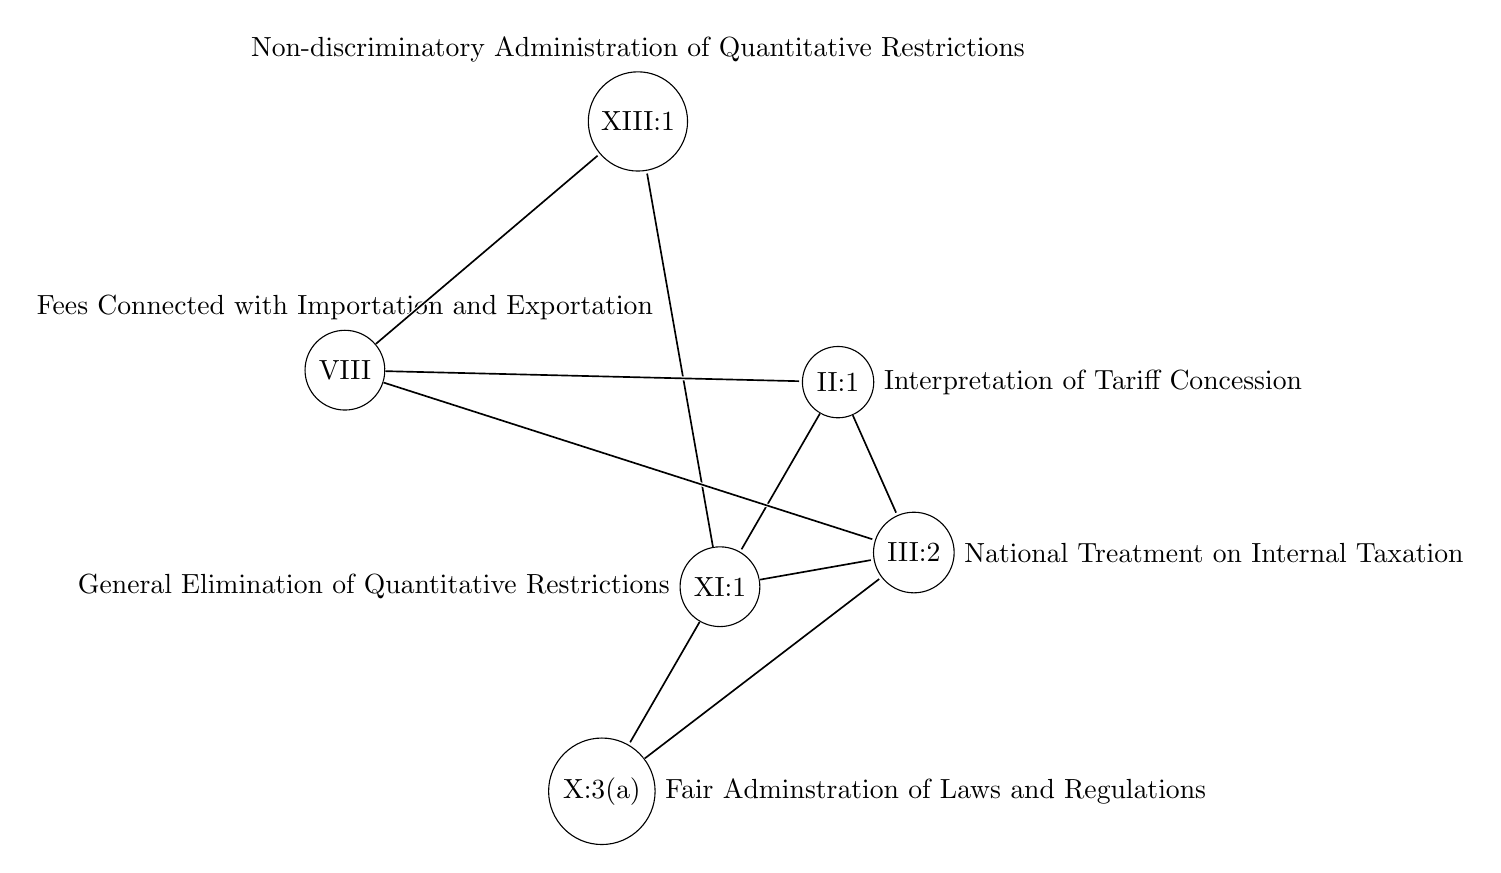
\begin{tikzpicture}[>={Stealth[color=black]},shorten >=1pt,node distance=2cm,on grid,initial/.style={}]
  \node[state, label=right:Interpretation of Tariff Concession] (T1) {II:1};
  \node[state, label=left:General Elimination of Quantitative Restrictions] at ([shift=({240:3 cm})]T1) (T4) {XI:1};
  \node[state, label=right:Fair Adminstration of Laws and Regulations] at ([shift=({240:3 cm})]T4) (T5) {X:3(a)};
  \node[state, label=above:Non-discriminatory Administration of Quantitative Restrictions] at ([shift=({100:6 cm})]T4) (T7) {XIII:1};
  \node[state, label=right:National Treatment on Internal Taxation] at ([shift=({10:2.5 cm})]T4) (T6) {III:2};
  \node[state, label=above:Fees Connected with Importation and Exportation] at ([shift=({150:5.5 cm})]T4) (T8) {VIII};

  \begin{scope}[every edge/.append style={-, double=black, draw=white}] % for directed edge, change "style={->, double=black, draw=white}]"
    \path (T1)
    edge   (T4)
    edge   (T6);
    \path (T4)
    edge   (T5)
    edge   (T6)
    edge   (T7);
    \path (T5)
    edge   (T6);
    \path (T8)
    edge   (T7)
    edge   (T1)
    edge   (T6);

  \end{scope}
\end{tikzpicture}

% to draw the node's border w/ color, refer to https://tex.stackexchange.com/questions/438412/how-to-add-border-to-a-node
  }
  \caption{Market Access}
  \label{fig:f2}
\end{figure}


% == END
\end{document}